%
\documentclass[11pt]{thesis} % draft

\title{Algorithmic Meta-Creativity}
\author{Fania Raczinski}
\date{March 2015}

\usepackage{lipsum}

\begin{document}

\lipsum[2]




% % Please add the following required packages to your document preamble:
% % \usepackage{booktabs}
% \begin{table}[]
% \centering
% \caption{My caption}
% \label{my-label}
% \begin{tabular}{@{}lll@{}}
% \toprule
% File & Words  & Lang \\ \midrule
% 00   & 22230  & e    \\
% 01   & 419456 & e    \\
% 02   & 33078  & e    \\
% 03   & 26843  & e    \\
% 04   & 103637 & f    \\
% 05   & 3853   & e    \\
% 06   & 134328 & f    \\
% 07   & 39937  & f    \\
% 08   & 4548   & f    \\
% 09   & 11309  & f    \\
% 10   & 110518 & e    \\
% 11   & 31286  & g    \\
% 12   & 78983  & f    \\
% 13   & 75293  & f    \\
% 14   & 20371  & e    \\
% 15   & 21822  & f    \\
% 16   & 54747  & e    \\
% 17   & 110980 & e    \\
% 18   & 0      &      \\
% 19   & 301903 & e    \\
% 20   & 0      &      \\
% 21   & 0      &      \\
% 22   & 14627  & f    \\
% 23   & 5873   & g    \\
% 24   & 12660  & f    \\
% 25   & 6647   & e    \\
% 26   & 8065   & e    \\
% 27   & 85467  & e    \\ \bottomrule
% \end{tabular}
% \end{table}




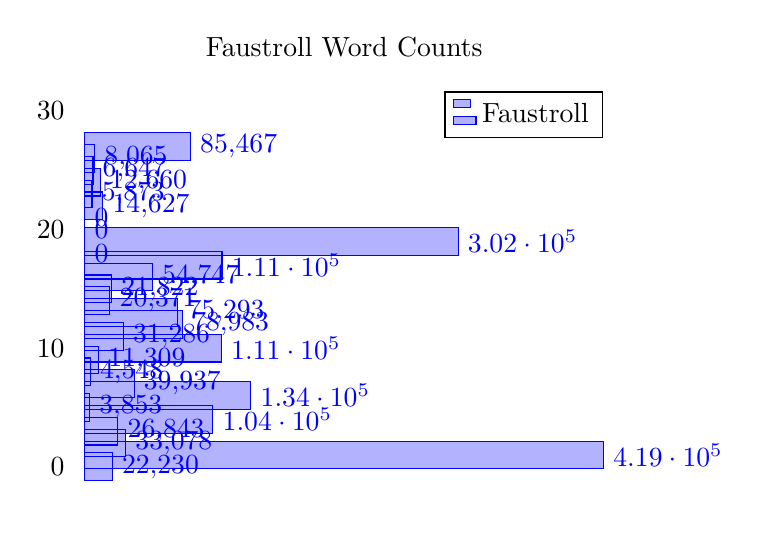
\begin{tikzpicture}
  \begin{axis}[title  = Faustroll Word Counts,
    xbar,
    y axis line style = { opacity = 0 },
    axis x line       = none,
    tickwidth         = 0pt,
    enlarge y limits  = 0.2,
    enlarge x limits  = 0.02,
    % symbolic y coords = {LaTeX, Tools, Distributions, Editors},
    nodes near coords,
  ]
  \addplot coordinates { 
  (22230, 0)
  (419456, 1)
  (33078, 2)
  (26843, 3)
  (103637, 4)
  (3853, 5)
  (134328, 6)
  (39937, 7)
  (4548, 8)
  (11309, 9)
  (110518, 10)
  (31286, 11)
  (78983, 12)
  (75293, 13)
  (20371, 14)
  (21822, 15)
  (54747, 16)
  (110980, 17)
  (0, 18)
  (301903, 19)
  (0, 20)
  (0, 21)
  (14627, 22)
  (5873, 23)
  (12660, 24)
  (6647, 25)
  (8065, 26)
  (85467, 27)            
  };
  % \addplot coordinates { (14320,LaTeX)         (1615,Tools)
                        %  (560,Distributions)   (3075,Editors)  };
  \legend{Faustroll}
  \end{axis}
\end{tikzpicture}


% \documentclass{article} 
% \usepackage{pgfplots}
% \begin{document}
% \begin{tikzpicture}
%   \begin{axis}[title  = Faustroll Word Count,
%     xbar,
%     y axis line style = { opacity = 0 },
%     axis x line       = none,
%     height			  = \textheight,
%     width			  = \textwidth,
%     tickwidth         = 0pt,
% %     enlarge y limits  = 0.2,
%     enlarge x limits  = 0.02,
%     nodes near coords,
%   ]
%   \addplot coordinates { 
%   (22230, 0)
%   (419456, 1)
%   (33078, 2)
%   (26843, 3)
%   (103637, 4)
%   (3853, 5)
%   (134328, 6)
%   (39937, 7)
%   (4548, 8)
%   (11309, 9)
%   (110518, 10)
%   (31286, 11)
%   (78983, 12)
%   (75293, 13)
%   (20371, 14)
%   (21822, 15)
%   (54747, 16)
%   (110980, 17)
%   (0, 18)
%   (301903, 19)
%   (0, 20)
%   (0, 21)
%   (14627, 22)
%   (5873, 23)
%   (12660, 24)
%   (6647, 25)
%   (8065, 26)
%   (85467, 27)            
%   };
% %   \addplot coordinates {
% %   (14320, 0)
% %   (17742, 1)
% %   (24371, 2)
% %   (26460, 3)
% %   (22812, 4)
% %   (16200, 5)
% %   (29213, 6)
% %   (28786, 7)
% %   (32031, 8)
% %   (25721, 9)
% %   (27631, 10)
% %   (27447, 11)
% %   (22776, 12)
% %   (26784, 13)
% %   (25833, 14)
% %   (25817, 15)
% %   (21704, 16)
% %   (20870, 17)
% %   (27513, 18)
% %   (22887, 19)
% %   (18233, 20)
% %   (22873, 21)
% %   (22254, 22)
% %   (23360, 23)
% %   (17233, 24)
% %   (22450, 25)
% %   (27866, 26)
% %   (23297, 27)
% %   (31090, 28)
% %   (25864, 29)
% %   (22159, 30)
% %   (17415, 31)
% %   (19634, 32)
% %   (21634, 33)
% %   (27537, 34)
% %   (21153, 35)
% %   (18293, 36)
% %   (25949, 37)
% %   (2568, 38)
% %   };
% %   \legend{Faustroll}
%   \end{axis}
% \end{tikzpicture}
% \end{document}

\end{document}
